\documentclass[12pt,a4paper]{article}
\usepackage[utf8]{inputenc}
\usepackage[english]{babel}
\usepackage{amsmath}
\usepackage{amsfonts}
\usepackage{amssymb}
\usepackage{graphicx}
\usepackage{hyperref}
\usepackage{xcolor}
\usepackage{listings}
\usepackage{caption}
\usepackage{subcaption}

\newcommand\todo[1]{\textcolor{red}{TODO: #1}}

\setlength\parindent{0pt}

\author{slarticodefast \\ \href{https://github.com/slarticodefast}{github.com/slarticodefast}}
\title{SS14 gas pump proposal}

\numberwithin{equation}{section}

\begin{document}
\maketitle
\begin{abstract}
	This document is intended to serve as a design document for improved gas pump mechanics following proper physics. We will derive the necessary formulas needed for an implementation from the basic laws of thermodynamics.
\end{abstract}

\todo{problems with current implementation of gas pumps: \\ no energy conservation, no soft clogging, arbitrary prioritization of one pump over another at low pressure, how does this fit into the atmos road map?}

\section{Ideal gases}

Space station 14 uses ideal gases to simulate atmospherics. An ideal gas is defined by following the ideal gas law

\begin{equation}
pV=nRT,
\end{equation}
where $p$ is the pressure in $kPa$, $V$ is the volume in $L$, $n$ is the amount of substance of gas in $mol$ with $1 mol=6.02214076 \cdot 10^{23}$ particles, $R = 8.314462618\cdot L \cdot kPa \cdot K^{-1} \cdot mol^{-1}$ is the universal gas constant and $T$ is the absolute temperature in $K$.
The internal energy of an ideal gas is defined by
\begin{equation}
U(n,T)=c_V n T,
\label{eqn:UcnT}
\end{equation}
where $c_V$ is the molar heat capacity at constant volume, defined in \texttt{gases.yml} for all in-game gases.

\section{First law of thermodynamics}
The first law of thermodynamics is a formulation of energy conservation
\begin{equation}
\Delta U = Q + W,
\end{equation}
where $\Delta U$ is the change in internal energy of the gas, $Q$ the heat supplied or withdrawn from the system and $W$ the work done on or by the system.
We use the positive sign convention, where all net energy transfers to the system are positive and all net energy transfers from the system are negative.
For an infinitesimally small change it takes the form
\begin{equation}
d U = \delta Q +\delta W,
\end{equation}
where the work $\delta W = -p dV$ can be calculated from the pressure $p$ and change in volume $dV$.

\section{Free expansion}
\begin{figure}[h]
\centering
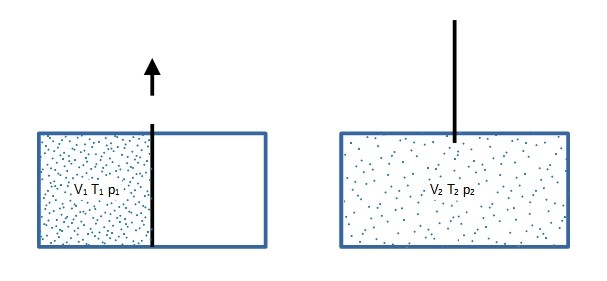
\includegraphics[scale=0.8]{image1}
\caption{Free expansion}
\label{fig:freeexp}
\end{figure}

\begin{figure}[h]
\centering
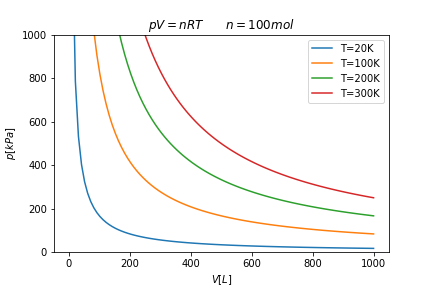
\includegraphics[scale=0.6]{plot1}
\caption{Lines of constant temperature (isothermals)}\label{fig:isothermalexp}
\end{figure}

If we let a gas expand freely by removing a barrier (\autoref{fig:freeexp}), no work is being done $W=0$ and no heat is exchanged with the outside of the (thermally isolated) box $Q=0$. Therefore the internal energy of the gas does not change $\Delta U = 0$. From \ref{eqn:UcnT} we follow that the temperature of the gas stays constant. We get
\begin{equation}
pV=nRT=const.
\end{equation}
or equivalently
\begin{equation}
p_1 V_1 =p_2 V_2, \qquad T_1=T_2, \qquad n_1=n_2.
\end{equation}
This process is not reversible as the gas cannot be forced back into the left part of the box without applying work.
In SS14 free expansion happens if you fill an empty pipe network with a gas, for example by opening a valve or using a connector port.
\newpage
\section{Adiabatic process}
\begin{figure}[h]
\centering
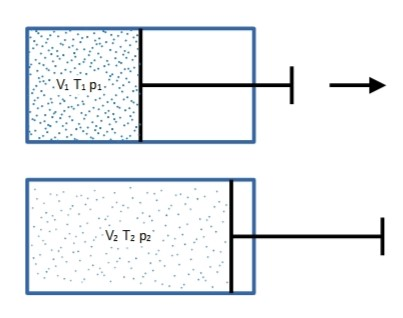
\includegraphics[scale=0.8]{image2}
\caption{Adiabatic expansion}\label{fig:adiabaticexp}
\end{figure}

Now we expand the gas using a piston instead (\autoref{fig:adiabaticexp}). The gas exchanges no heat with the environment outside the box and we have $\delta Q=0$. The gas presses against the side of the piston as it expands, doing the work $\delta W = -pdV$. We get
\begin{align}
c_VndT=dU&=\delta W\\
&= -pdV.
\end{align}

Using the product rule of differentiation we get
\begin{align}
dT&=d\Big(\frac{pV}{nR}\Big)\\
&=\frac{1}{nR} d(pV)\\
&=\frac{1}{nR} (pdV+Vdp)
\end{align}
leading to
\begin{align}
&&\frac{c_V}{R}(pdV+Vdp)&=-pdV&\\
&\iff&-\Big(\frac{c_V+R}{c_V}\Big) pdV&=Vdp&\\
&\iff&-\gamma \frac{dV}{V}&=\frac{dp}{p}&
\end{align}
with the heat capacity ration $\gamma = \frac{c_p}{c_v}=\frac{c_V+R}{c_V}$. This value is already defined for all gases in \texttt{gases.yml}, but currently unused. Integrating both sides gives us
\begin{align}
-\gamma \ln \Big( \frac{V_2}{V_1} \Big) =\ln \Big( \frac{p_2}{p_1} \Big)
\end{align}
and exponentiating  gives us
\begin{equation}
\Big( \frac{V_2}{V_1} \Big)^{-\gamma} = \frac{p_2}{p_1}.
\end{equation}
By inserting the ideal gas law we finally get
\begin{align}
p_1V_1^\gamma&=p_2V_2^\gamma&=const.&&\\
p_1^{1-\gamma}T_1^\gamma&=p_2^{1-\gamma}T_2^\gamma&=const.&&\\
T_1V_1^{\gamma-1}&=T_2V_2^{\gamma-1}&=const.&&
\end{align}


This process is reversible, which means we can compress the gas adiabatically and get back to the initial state using the same formula.
To calculate the total work done during the process we use
\begin{align}
W &= -\int_{V_1}^{V_2} p dV\\
&= -\int_{V_1}^{V_2} p_1 \Big(\frac{V_1}{V}\Big)^\gamma dV\\
&= -p_1 V_1^\gamma \Big[\frac{1}{\gamma-1}V^{1-\gamma}\Big]_{V_1}^{V_2}\\
&=\frac{V_1 p_1 - V_2 p_2}{\gamma-1}.
\end{align}
For compression this value is positive, for expansion negative.

\section{Mixtures of ideal gases}
We now combine different ideal gases in a setup similar to \autoref{fig:freeexp}, but with the second gas in the right chamber. The resulting gas mix will act as an ideal gas with the properties

\begin{align}
U_{mix} &= \sum\nolimits_i U_i\\
c_{V,mix} &= \frac{\sum_i n_i c_{V,i}}{\sum_i n_i}\\
T_{mix} &= \frac{\sum n_i c_{V,i}T_i}{\sum_i n_i c_{V,i}}\\
V_{mix} &= \sum\nolimits_i V_i\\
\gamma_{mix} &=\frac{\sum_i n_i c_{p,i}}{\sum_i n_i c_{V,i}}\\
&=\frac{\sum_i n_i (c_{V,i}+R)}{\sum_i n_i c_{V,i}}.
\end{align}
The internal energies and heat capacities are additive due to energy conservation. Note that merging a gas with an empty volume with $V_2>0$, $n_2=0$, $p=0$ is equivalent to free expansion.

\newpage
\section{Piston pump}
\begin{figure}[h]
\centering
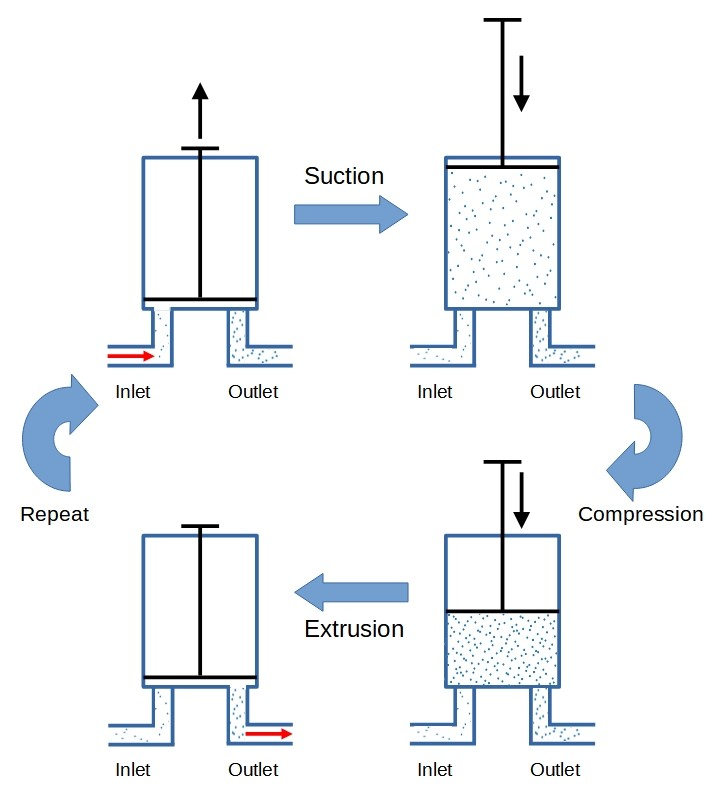
\includegraphics[scale=0.5]{image3}
\caption{Adiabatic expansion}\label{fig:piston}
\end{figure}

A simple piston pump has the following cycle (see \autoref{fig:piston}):
\begin{enumerate}
\item Suction: Open valve 1 and adiabatically expand the inlet gas from $V_{in}$ to $V_{in}+V_{pump}$. Then close valve 1, which splits off the volume $V_{pump}$ from the inlet gas.

\begin{align}
V_{in} \longrightarrow & V_{in}\\
n_{in} \longrightarrow & n_{in}\Big(\frac{V_{in}}{V_{in}+V_{pump}}\Big)\\
p_{in} \longrightarrow & p_{in}\Big(\frac{V_{in}}{V_{in}+V_{pump}}\Big)^{\gamma_{in}}&=p_{pump}\\
T_{in} \longrightarrow & T_{in}\Big(\frac{V_{in}}{V_{in}+V_{pump}}\Big)^{\gamma_{in}-1}&=T_{pump}\\
&n_{in}\Big(\frac{V_{pump}}{V_{in}+V_{pump}}\Big)&=n_{pump}
\end{align}
\item Compression: Adiabatically compress the gas inside the pump from until it equals the output pressure. This step can be skipped if the output pressure is lower than the pressure inside the pump.

\begin{align}
V_{pump} &\longrightarrow V_{pump} \Big(\frac{p_{pump}}{p_{out}} \Big)^{\frac{1}{\gamma_{in}}}&= V'_{pump}\\
n_{pump} &\longrightarrow n_{pump}\\
p_{pump} &\longrightarrow p_{out}\\
T_{pump} &\longrightarrow T_{pump}\Big(\frac{p_{pump}}{p_{out}} \Big)^{\frac{1-\gamma_{in}}{\gamma_{in}}}&= T'_{pump}
\end{align}
\item Extrusion: Open valve 2, causing the pump gas and outlet gas to mix, then compress the mixed gas adiabatically from $V_{out} + V'_{pump}$ to $V_{out}$ by moving the piston to its initial position. Close valve 2 and the cycle can restart.

\begin{align}
V_{out}+V'_{pump} \longrightarrow & V_{out}\\
n_{mix} \longrightarrow & n_{mix}\\
p_{out} \longrightarrow & p_{out}\Big(\frac{V_{out}+V'_{pump}}{V_{out}}\Big)^{\gamma_{mix}}\\
T_{out} \longrightarrow & T_{out}\Big(\frac{V_{out}+V'_{pump}}{V_{out}}\Big)^{\gamma_{mix}-1}
\end{align}
\end{enumerate}
\todo{Sum of work done for all three steps of the cycle. Find closed form solution to limit the pump volume $V_{pump}$ by the pumps power usage.}
\\
We have two types of pumps in SS14: One is the volume pump, which has a maximum output pressure of $9000 kPa$ and a selectable transfer volume per cycle. The other one is the pressure pump, which has an infinite maximum transfer volume, but only transfers gas up to a selectable output pressure (maximum $4500kPA$).
\\
For the pump rework we would make both pumps work as described above with one cycle in each update step. The pressure pump should pump until a certain pressure threshold is met and then stop, but have a constant (but maybe higher) internal pump volume. The volume pump should have the internal pump volume $V_{pump}$ be selectable like before, but have no maximum output pressure. If we limit the pumps throughput by its maximum energy usage, its effectiveness will be reduced at high pressure. These diminishing returns will stop the player from creating extremely high-pressured areas. Breaking pipes at extremely high pressures has also been suggested in the atmos roadmap.

\section{Examples}
\begin{figure}[h]
\centering
   	\begin{subfigure}{.45\textwidth}
    \centering
	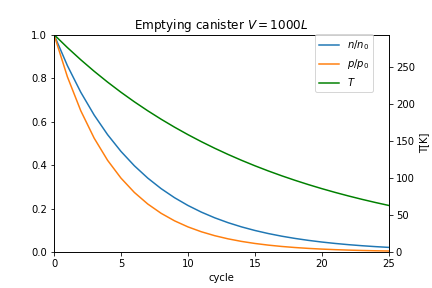
\includegraphics[scale=0.45]{plot2}
	\end{subfigure}
   	\begin{subfigure}{.45\textwidth}
    \centering
	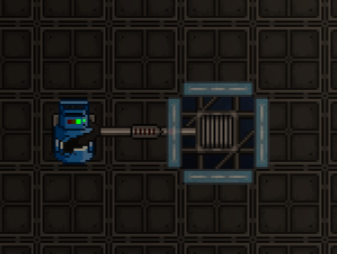
\includegraphics[scale=0.52]{screen1}
	\end{subfigure}
\caption{Removing gas from a canister}
\label{fig:vacuum}
\end{figure}
\begin{itemize}
\item Lowering the pressure in a gas container using a pump will now properly cool down the gas. The effects of the adiabatic expansion are shown in \autoref{fig:vacuum}. The pumps efficiency becomes lower with lower input pressure. The gas amount inside will decay exponentially, meaning that most of the gas can be removed quickly and the remaining trace amounts should not matter for any practical purposes. If you want to completely empty a container quickly you will have to connect it to space.
\item Filling an empty pipe network with gas using a pump will not cause it to cool down since it is a free expansion. However, compressing it to a pressure higher than that of the pump input will cause it to heat up. This is good from a gameplay perspective: Atmos techs can no longer 'overclock' distro by making it extremely high pressure without also regulating the temperature. Leaving it at normal pressure won't influence the temperature and requires no additional setup. \todo{diagram}
\end{itemize}

\section{Implementation notes}
\begin{itemize}
\item The pressure is a computed property in the \texttt{GasMixture} class and is only calculated when needed using $pV=nRT$.
\item All the basic thermodynamic processes for gases should have a corresponding function in \texttt{AtmosphereSystem.Gases.cs}. Any state change done to gases falls into one of these categories, so this can prevent a lot of code duplication.
\item The \texttt{Merge} function in  \texttt{AtmosphereSystem.Gases.cs} should be renamed as it does not merge two gas mixtures, but instead only transfers the heat and moles from one gas to another, ignoring the volume. A new merge function should be written which properly combines two gas mixtures while adding their volume. This is often needed, for example when opening valves or connecting pipe networks when building. With this more code duplication can be prevented.
\item Due to to the theorem of equipartition of energy an ideal gas should have the molar heat capacity $c_{v,m}=\frac{1}{2}fR$ where $f$ is the number of degrees of freedom of the molecule. For a monoatomic ($f=3$, $3$ translational d.o.f.), diatomic ($f=5$, $3$ translational and $2$ rotational d.o.f.) and triatomic ($f=5$, $3$ translational and $3$ rotational d.o.f.) ideal gas this would result in $c_{V,m}=\frac{3}{2}R$, $\frac{5}{2}R$ and $\frac{6}{2}R$ respectively. Our gases have different values meaning they do not behave like an ideal gas in all cases.
\item Pumps currently run 8 times faster than shown to the player. This speedup is set in the \texttt{atmos.speedup} cvar. So if a volume pump is set to $200 L/s$ it actually pumps $1600 L/s$, which is not shown to the player. This should be corrected by either removing the cvar or showing the correct speed in the clients interface. Also for energy conservation reasons the speedup should not be able to circumvent the maximum transfer speed given by the pumps power usage.
\item Currently filters and gas mixers also work as pumps. These will be changed to be flow based according to the atmos roadmap. This should probably be merged at the same time as this proposal.
\item \todo{Automatically calculate $\gamma$ from $\gamma=\frac{c_{p,m}}{c_{v,m}}=\frac{c_{v,m}+R}{c_{v,m}}$ instead of using a datafield? Possibly necessary for energy conservation? Check the physics of non-ideal gases for that.}
\end{itemize}


%\bibliographystyle{plain}
%\bibliography{pumps}
\end{document}